\documentclass[11pt]{article}
\usepackage[a4paper,top=0.6cm,bottom=3.0cm,left=1.9cm,right=1.9cm,footskip=2.0cm]{geometry}
\usepackage{graphicx}
\usepackage[table]{xcolor}
\usepackage{ragged2e}
\usepackage{fancyhdr}
\usepackage{fontspec}
\setmainfont{Noto Sans Bengali}
\setsansfont{Noto Sans Bengali}
\newfontfamily\latinfont{Carlito}
\renewcommand{\familydefault}{\sfdefault}
\definecolor{titleblue}{HTML}{0F2F4A}
\definecolor{textblack}{HTML}{1A1A1A}
\definecolor{rule}{HTML}{C9C4C0}
\definecolor{muted}{HTML}{6B635E}
\setlength{\parindent}{0pt}\setlength{\parskip}{0.5em}

\setlength{\headheight}{28pt}\setlength{\headsep}{6pt}
\newcommand{\idmfooter}{%
  \begin{minipage}{\textwidth}
    {\color{rule}\hrule height 0.7pt}\vspace{4pt}
    \noindent
    \begin{minipage}[c]{0.66\textwidth}{\scriptsize\color{muted}{\latinfont Developed by the Water and Climate Lab, IIT Gandhinagar, using hydro-meteorological data from partner agencies}.}\end{minipage}\hfill
    \begin{minipage}[c]{0.32\textwidth}\raggedleft
      
\includegraphics[height=0.62cm]{wcl.png}\hspace{6pt}%
      
\includegraphics[height=0.62cm]{iitgn.png}
    \end{minipage}\\[3pt]
    {\scriptsize\color{muted}© {\latinfont 2026 Water and Climate Lab} · {\latinfont Indian Institute of Technology Gandhinagar} · {\latinfont For research and demonstration purposes}.}
  \end{minipage}%
}
\newcommand{\idmrunhead}{%
  \begin{minipage}{\textwidth}
    {\small\bfseries\color{titleblue}{\latinfont National Drought Summary}}\hfill{\small\color{muted}{\latinfont Week ending May 20, 2026}}\\[2pt]
    {\color{rule}\hrule height 0.6pt}
  \end{minipage}%
}
\fancypagestyle{idmfoot}{\fancyhf{}\renewcommand{\headrulewidth}{0pt}\renewcommand{\footrulewidth}{0pt}\fancyfoot[C]{\idmfooter}}
\fancypagestyle{idmrun}{\fancyhf{}\renewcommand{\headrulewidth}{0pt}\renewcommand{\footrulewidth}{0pt}\fancyhead[C]{\idmrunhead}\fancyfoot[C]{\idmfooter}}
\pagestyle{idmrun}

\begin{document}

\thispagestyle{idmfoot}
\noindent
\begin{minipage}[c]{0.16\textwidth}
\includegraphics[width=\linewidth]{wcl.png}\end{minipage}\hfill
\begin{minipage}[c]{0.80\textwidth}\raggedleft
  {\fontsize{19}{22}\selectfont\bfseries\color{titleblue}{\latinfont National Drought Summary}}\\[2pt]
  {\normalsize\color{muted}{\latinfont Week ending May 20, 2026}}
\end{minipage}
\vspace{6pt}{\color{rule}\hrule height 1pt}\vspace{10pt}
\begin{center}
  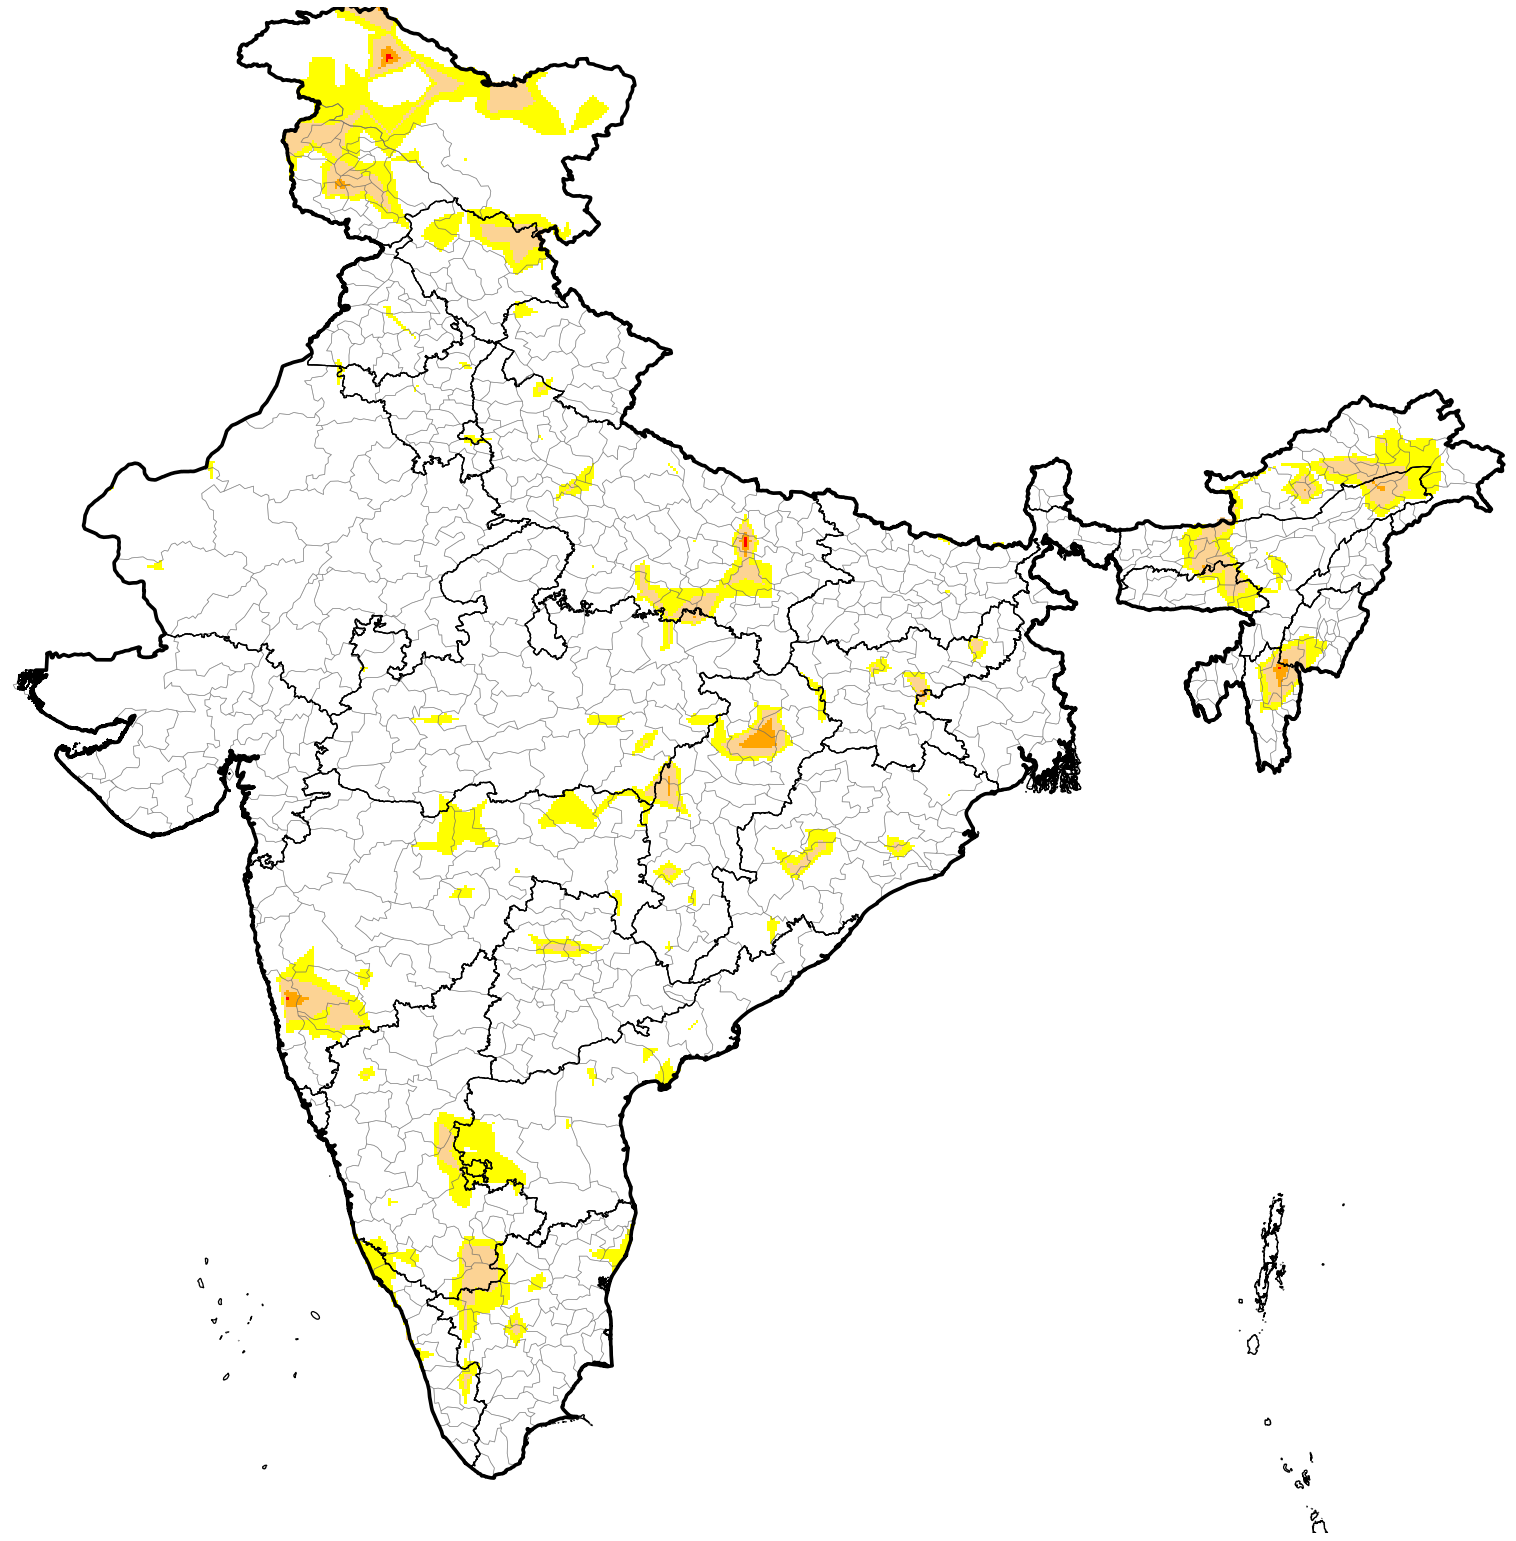
\includegraphics[width=0.60\textwidth]{cdi_map.png}\\[3pt]
  {\small\color{muted}{\latinfont Combined Drought Index (CDI) for the week ending May 20, 2026}.}
\end{center}
\vspace{2pt}
{\large\bfseries\color{titleblue}{\latinfont Summary}}\\[3pt]
{\justifying\normalsize\color{textblack}এই সপ্তাহত ৰাষ্ট্ৰীয় খৰাংৰ পৰিস্থিতিৰ বৈশিষ্ট্য হৈছে অধিকাংশ অঞ্চল সাধাৰণ শ্ৰেণীত থাকিব, কিছু অংশত খৰাংৰ অৱস্থা। এই সপ্তাহত ভাৰতৰ ১৫.৩ শতাংশ অঞ্চল ডি০ বা তাৰ নিম্নত বৰ্ণিত। এই সংখ্যাটো বিগত সপ্তাহৰ তুলনাত হ্ৰাস, কাৰণ সপ্তাহৰ পৰা সপ্তাহলৈ খৰাং অঞ্চল ০.৯ শতাংশ বিন্দুমত হ্ৰাস পাইছে। খৰাংৰ প্ৰভাৱত আটাইতকৈ বেছি প্ৰভাৱিত অঞ্চলসমূহ হ'ল দিল্লী ছিট, মণিপুৰ, মিজোৰাম, অৰুণাচল প্ৰদেশ, জম্মু কাষ্মिर আৰু মেঘালয়। আনহাতে পশ্চিম বংগ ০.০ শতাংশ অঞ্চলত খৰাং দেখাৱলৈ জনাইছে, আৰু ৰাজস্থান, গুজৰাট আৰু তেলেংগানা প্ৰতিটোৱে নিজৰ অঞ্চলৰ যথাক্রমে ১.০ শতাংশ, ২.১ শতাংশ আৰু ৩.৪ শতাংশত খৰাং দেখাৱলৈ জনাইছে।\par}
\vspace{8pt}
{\large\bfseries\color{titleblue}{\latinfont Regional Outlook}}\\[2pt]
{\normalsize\color{titleblue}\textbf{{\latinfont North}}}\enspace {\normalsize\color{textblack}{\latinfont Moderate, scattered drought. About 28}\% {\latinfont of the area is in drought (D0}–{\latinfont D4)}.} \par\smallskip {\normalsize\color{titleblue}\textbf{{\latinfont Northwest}}}\enspace {\normalsize\color{textblack}{\latinfont Largely normal conditions. About 4}\% {\latinfont of the area is in drought (D0}–{\latinfont D4)}.} \par\smallskip {\normalsize\color{titleblue}\textbf{{\latinfont Northeast}}}\enspace {\normalsize\color{textblack}{\latinfont Moderate, scattered drought. About 27}\% {\latinfont of the area is in drought (D0}–{\latinfont D4). Pockets of severe-or-worse conditions are present}.} \par\smallskip {\normalsize\color{titleblue}\textbf{{\latinfont East}}}\enspace {\normalsize\color{textblack}{\latinfont Mostly normal, with localised dryness. About 7}\% {\latinfont of the area is in drought (D0}–{\latinfont D4)}.} \par\smallskip {\normalsize\color{titleblue}\textbf{{\latinfont Central}}}\enspace {\normalsize\color{textblack}{\latinfont Mostly normal, with localised dryness. About 15}\% {\latinfont of the area is in drought (D0}–{\latinfont D4). Pockets of severe-or-worse conditions are present}.} \par\smallskip {\normalsize\color{titleblue}\textbf{{\latinfont West}}}\enspace {\normalsize\color{textblack}{\latinfont Moderate, scattered drought. About 22}\% {\latinfont of the area is in drought (D0}–{\latinfont D4)}.} \par\smallskip {\normalsize\color{titleblue}\textbf{{\latinfont South}}}\enspace {\normalsize\color{textblack}{\latinfont Mostly normal, with localised dryness. About 16}\% {\latinfont of the area is in drought (D0}–{\latinfont D4)}.}
\end{document}
